\documentclass[12pt]{article}
\usepackage{fullpage}
\usepackage[margin=1in]{geometry}
\usepackage[stable]{footmisc}
\usepackage{graphicx}
\usepackage{amssymb}
\usepackage{IEEEtrantools}
\usepackage{lineno}
\usepackage{amsmath}
\usepackage{epstopdf}
\usepackage{parskip}
\usepackage{authblk}
\usepackage[authoryear]{natbib}
%\setlength{\parskip}{20pt}
\linespread{1.6}
\date{}

\DeclareGraphicsRule{.tif}{png}{.png}{`convert #1 `dirname #1`/`basename #1 .tif`.png}


%%	math short-cuts
\def \ve{\varepsilon}	% epsilon used for metabolic rate
\def \la{\lambda}	% lambda
\newcommand{\eref}[1]{(\ref{#1})}

%%	new commands for referencing figures and tables and sections
\newcommand{\fref}[1]{Figure~\ref{#1}}	% inline figure ref
\newcommand{\fpref}[1]{Fig.~\ref{#1}}	% parenthetical figure ref
\newcommand{\tref}[1]{Table~\ref{#1}}	% table ref
\newcommand{\sref}[1]{Section~\ref{#1}}	% table ref
%\linenumbers

\title{\Large \textbf{Growth with MERA: a dynamic resource constraint}}

\author{Jade, Oct 16}

\begin{document}
\maketitle
\raggedright
\large
\setlength{\parindent}{15pt}

One reason why the current MERA framework does not lead to a realistic growth function is that it assumes all resources can be potentially utilized by the individuals currently existing in the community, even if there is only a few individuals. This contradicts the reality that the amount of resource acquired by the species has to be limited by its abundance, both through the limited ability to utilize resource for each individual (upper bound for metabolism and reproductivity) and the decreased probability for a small number of individuals to get a large amount of resource. Here I am going to address this limit by adding one more step before resource allocation happens among species and individuals: the community-level resource acquisition step. Given the maximal resource acquisition of the current community (regulated by the abundance) and the total resource available in the environment, this step determines dynamically at each step how much total resource the community can get, i.e. the resource constraint for the previous MERA allocation. This is realized by maximizing the number of microstates in mapping resource units in the environment to resource units actually utilized, based on the same principle used in the original MERA framework. For a simple one species case (under two scenarios for resource redistribution), this extra step gives growth functions that highly resembles the logistic growth function but with some unique properties that can be tested with data.

\section{Community-level resource acquisition}

Our question is, when there is a constant resource available in the environment ($R_0$) and meanwhile the community has an upper limit to the amount of resource it can utilize, how much resource it can actually get. To address this let's first consider a similar problem: there are $X$ boxes and $Y$ balls; the boxes can each contain at most one ball. If I randomly throw balls into the boxes (and assume that the probability of a given ball to be thrown into any box or out of all boxes follows a uniform distribution), what is the most likely number of boxes that have balls in them? It is easy to see that this number can not be bigger than $X$, since that is the upper limit of number of boxes; it also cannot be bigger than $Y$, since there are $Y$ balls in total. We can also infer that when $Y$ is much bigger than $X$, the most likely number of boxes with balls in it will be close to $X$ (since the chance of any one box not being occupied after a large number of throws is very low), and similarly when $X$ is much bigger than $Y$, this number will be close to $Y$ (since given a large number of boxes, the probability of not being thrown into any of them is very low). But what is the most likely value for any given $X$ and $Y$? In the following I will show that this value can also be determined by maximizing the number of microstates.

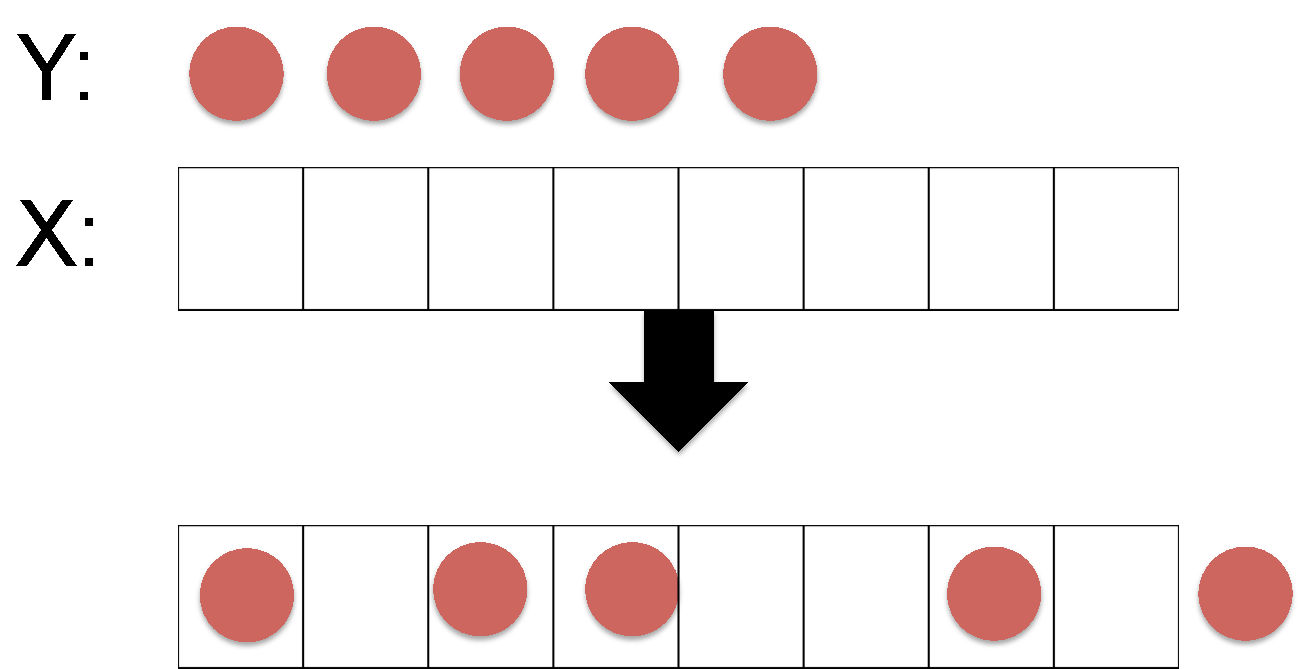
\includegraphics[width=0.6\textwidth]{XY_demo.pdf}

(Notice the boxes and balls should be regarded as distinguishable.)

Let's define the number of actually occupied boxes to be $R$. For any given $X$ and $Y$, if we take a certain value of $R$ to be the macrostate, the microstate can be defined as a particular way to match balls with boxes. The number of microstates for the macrostate $R$ can be expressed by:
 
  \begin{equation}
 \begin{split}
W(R,X,Y) = C(R,X-R|X) \times C(R,Y-R|Y)
\end{split}
\end{equation}

$C$ is the combination function:
\begin{equation}
C(x_1,x_2,... |X) = \frac{X!}{x_1! x_2! ...}
\end{equation}
So the number of microstates is the number of ways to select $R$ balls from $Y$ balls times the number of ways to select $R$ boxes out of $X$ boxes to contain these balls. With Sterling's approximation we can get:
  \begin{equation}
 \begin{split}
\mbox{log} W(R,X,Y) = X \mbox{log} X + Y \mbox{log} Y - 2 R \mbox{log} R \\
 - (X-R) \mbox{log} (X-R) - (Y-R) \mbox{log} (Y-R)
\end{split}
\end{equation}
Take the derivative over $R$ and set it to zero:

  \begin{equation}
 \begin{split}
\frac{\partial \mbox{log} W(R,X,Y)}{\partial R} =  - 2 \mbox{log} R + \mbox{log} (X-R) + \mbox{log} (Y-R) = 0\\
=> R^2 = (X-R)(Y-R)\\
=> R = \frac{XY}{X+Y}
\end{split}
\end{equation}
Eq. 4 gives the most likely $R$ (that maximizes the number of microstates) for any $X$ and $Y$. We can see that it is smaller than both $X$ and $Y$; when $X$ is much bigger than $Y$, it is close to $Y$; when $Y$ is much bigger than $X$, it is close to $X$.

Now let's go back to our problem: what are the variables corresponding to $X$ and $Y$ in our scenario? There might be other interpretations but to me here is the most straightforward one: $X$ is the maximal resource the community could utilize given its current abundance, while $Y$ is the total resource available in the environment. Actually $X$ and $Y$ are symmetrical in Eq. 4 so it does not really matter if you switch their interpretations. The more important thing is to keep in mind that one of them represents  the potential of the community (the boxes) while the other represents the size of the resource supply (the balls). From these two the actual (most likely) amount of resource obtained by the community can be derived. After this value is determined, the previous resource allocation procedure can take it as the resource constraint and proceed to derive resource distributions among and within species. That is why I am not counting the number of permutations for balls in the boxes although I have assumed the boxes and balls to be distinguishable; which ball (resource unit) goes to which box (individual) should be determined by the resource allocation process. Here we only care about the total amount of resource for the whole community. 

Given this as the baseline, two scenarios can be developed to further determine the growth function given by this procedure.

\section{Two possible scenarios: partial vs complete redistribution}
In the last section I have showed the basic logic to dynamically determine the resource constraint for MERA allocation given the potential of the community and the resource supply. The next thing would be to determine the exact expressions of these two terms. There are two alternative ways to do it, based on the assumption of whether the resource units are fixed by the species once obtained; or all resource units (including those previously obtained by the species) must be redistributed in every step. I will call the former partial redistribution and the latter complete redistribution. In the below we will look at the partial scenario first.

\subsection{Partial redistribution}
Recall that in Eq. 4, $X$ is the maximal resource the community could utilize given its current abundance, while $Y$ is the total resource available in the environment. When resource is fixed to the population once obtained, the community-level resource acquisition only applies to the additional amount of resource the population gets, or the net growth in resource content of the species. If we define $r$ as the maximal per capita net growth rate (intrinsic growth rate), $X$ will be simply expressed by
  \begin{equation}
 \begin{split}
X = r N \theta 
\end{split}
\end{equation}
Eq. 5 is precisely the maximal amount of additional resource the population can utilize (corresponding to the maximal net growth rate). On the other hand for $Y$,
  \begin{equation}
 \begin{split}
Y = R_0 - \theta N
\end{split}
\end{equation}
which is amount of resource left in the environment available for the net growth (total resource available $R_0$ minus the amount that is preempted by the existing population). Plugging Eqs. 5 and 6 into Eq. 4 we have the expression for the most likely (corresponding the most number of microstates in community level resource acquisition) amount of resource obtained by the net growth of the population.
  \begin{equation}
 \begin{split}
R = \frac{r N \theta (R_0 - \theta N)}{R_0 + (r-1) N \theta}
\end{split}
\end{equation}
The most likely per capita net growth rate can then be determined by
  \begin{equation}
 \begin{split}
g = \frac{R}{\theta N} = \frac{r (R_0 - \theta N)}{R_0 + (r-1) N \theta}
\end{split}
\end{equation}
The steady state abundance $\hat{N}$ can be solved by setting $g$ to 0,
  \begin{equation}
 \begin{split}
 \hat{g} = \frac{R}{\theta \hat {N}} = \frac{r (R_0 - \theta \hat {N})}{R_0 + (r-1) \hat {N} \theta} = 0\\
=> \hat {N} = \frac{R_0}{\theta } 
\end{split}
\end{equation}
we can further transform Eq. 8 to be
  \begin{equation}
 \begin{split}
g =  \frac{r (1 - \frac{N}{\hat {N}})}{1 + (r-1) \frac{N}{\hat {N}}}
\end{split}
\end{equation}
We can see that the numerator in Eq. 10 is exactly logistic growth, but the denominator is not equal to 1 unless $r=1$. In other words, when the intrinsic growth rate of the population is 1, maximizing community-level resource acquisition microstates gives exactly the same prediction as the logistic growth function. However, in all other cases the predictions will be different.

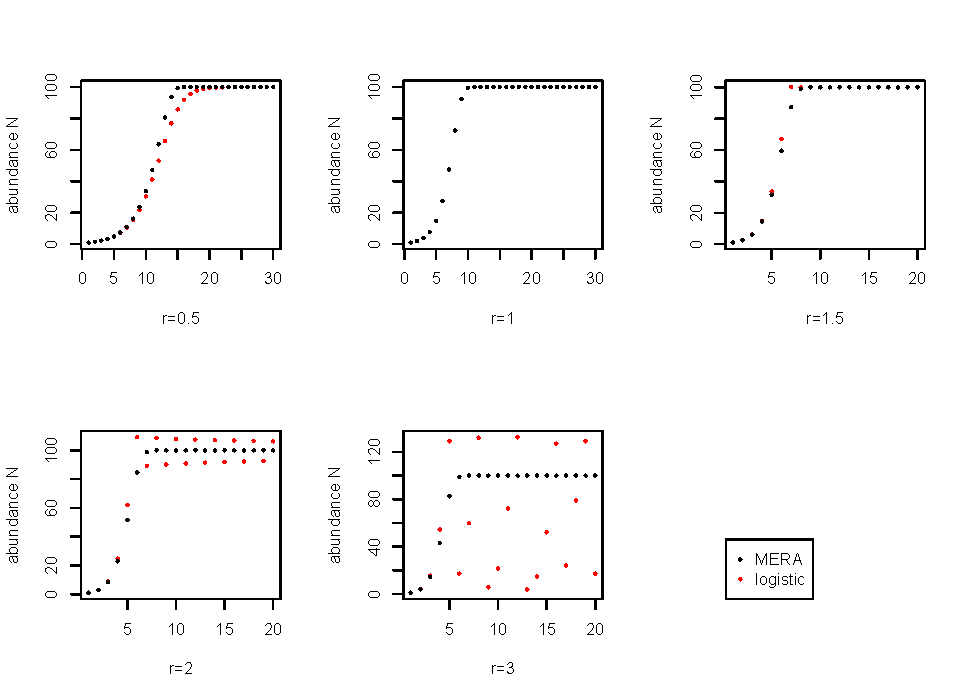
\includegraphics[width=\textwidth]{partial_result.pdf}

\begin{center}
Time (partial redistribution, $\hat {N} =100$)
\end{center}

We can see that when $r$ is smaller than 1, MERA predicts faster growth than the logistic growth function; when $r=1$, they overlap; when $r>1$, MERA prediction grows more slowly than the logistic function; moreover, there are no oscillations at large $r$ values. These properties are due to the additional density dependence imposed by the denominator term in Eq. 10. To me these are good properties; it never made sense to me why population could oscillate so wildly when $r=3$ (which is not that high for fecundity). Of course the actual goodness of fit has to be tested with data, but at a first sight I think MERA provides a more realistic discrete growth model than the logistic growth function.
  
\subsection{Complete redistribution}
In this scenario, resource cannot be fixed by the population and redistribution happens over the whole resource pool. Therefore community-level resource acquisition applies to not the additional amount, but the total amount of resource the population gets:
\begin{equation}
 \begin{split}
X = (r+1) N \theta 
\end{split}
\end{equation}
 $r$ is still the intrinsic growth rate but $X$ is the maximal amount of total resource the population can utilize. Correspondingly, since all resources are prone to redistribution, $Y$ is simply
 \begin{equation}
 \begin{split}
Y = R_0
\end{split}
\end{equation}
Then the most likely total resource for the population is 
 \begin{equation}
 \begin{split}
R = \frac{(r+1) N \theta  R_0}{(r+1) N \theta +R_0}
\end{split}
\end{equation}
From which the most likely per capita net growth can be derived:
 \begin{equation}
 \begin{split}
(1+g) \theta N = R = \frac{(r+1) N \theta  R_0}{(r+1) N \theta +R_0}\\
 = > g = \frac{(r+1) R_0}{(r+1) N \theta +R_0} -1
\end{split}
\end{equation}
The steady state abundance $\hat{N}$ can again be solved by setting $g$ to 0,
 \begin{equation}
 \begin{split}
\hat{g} = \frac{(r+1) R_0}{(r+1) \hat{N} \theta +R_0} -1 = 0\\
 = > \hat{N} = \frac{r R_0}{(r+1) \theta}
\end{split}
\end{equation}
We can see that in the complete redistribution scenario, the steady state abundance is smaller than that in the partial scenario. 

**Intuitively speaking, when resource can be fixed as in the partial scenario, given enough time all resources can be fixed by the population. Whereas if resource cannot be fixed, there will always be a non-zero proportion of the resource that is not obtained by the population, which is ensured by the maximization of microstates (number of microstates will be small if this proportion is zero).**

Plugging Eq. 15 back into Eq. 14, we have
 \begin{equation}
 \begin{split}
g = \frac{(r+1) R_0}{(r+1) N \theta +R_0} -1 = \frac{rR_0  - (r+1) N \theta }{R_0 + (r+1) N \theta} \\
= \frac{ r(1- N/\frac{r R_0}{(r+1) \theta})} {1+ r N/\frac{r R_0}{(r+1) \theta}} = \frac{ r(1- \frac{N }{\hat{N}})} {1+ r \frac{N }{\hat{N}}}
\end{split}
\end{equation}
The numerator is still the same as the logistic growth function, but this time the denominator is always a positive function of $N$ for all $r>0$. This means that there will always be stronger density dependence and slower growth than the logistic growth no matter what how big $r$ is (as long as it is positive). This is proved in following graphs.

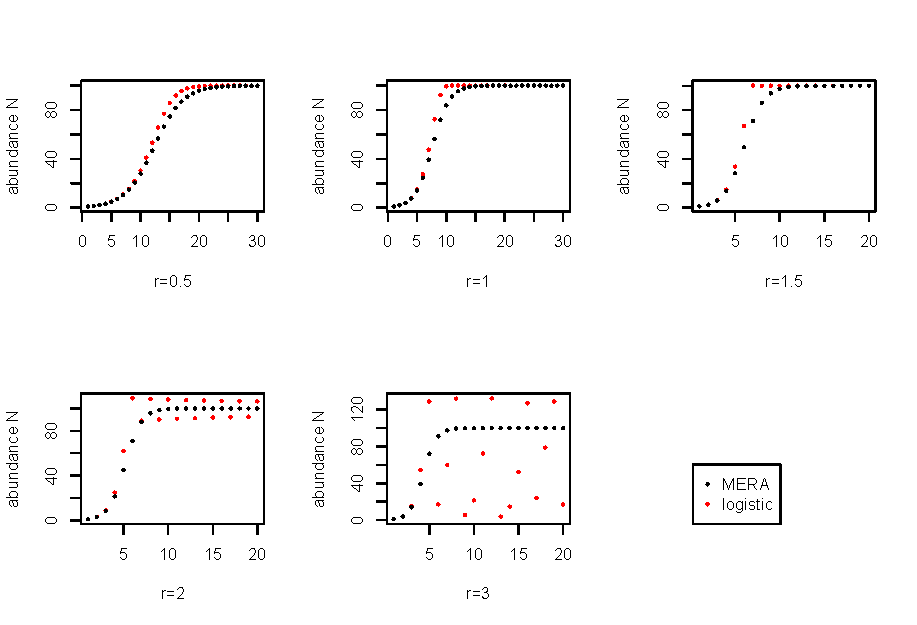
\includegraphics[width=\textwidth]{complete_result.pdf}

\begin{center}
Time (complete redistribution, $\hat {N} =100$)
\end{center}

\section{Discussions}
In this write-up an important issue in the previous MERA, i.e. a constant pre-defined resource constraint (and the associated assumption of infinite population growth potential), was addressed and along comes the MERA solution for single species growth function. Only the one species scenario is discussed here but this model can be applied to multiple species scenario. The resource constraint is now derived to be a function of the current community size under the same framework of maximizing microstates. After this first step, resource allocation can in turn determine the resource distributions among and within species as in the previous framework. The underlying assumption is that community-level resource acquisition is independent of within-community resource allocation, other than determining the resource constraint for the latter. 

Although not exclusively, the partial redistribution scenario more intuitively applies to stock resources, where the resources can be maintained and recycled within the population; while the complete redistribution scenario more intuitively applies to flow resources, where resources cannot be maintained or recycled but have to be actively acquired from the environment each time.

Since we are using the constrained MERA for resource allocation, for the one species case, individual distinguishability ($D_r$) does not affect the resource it gets (it has to utilize all resources acquired from the community-level resource acquisition). When there are more than one species, individual distinguishability will potentially affect the growth function. But to start with, we should test the one species growth functions first.

The growth functions derived from this approach have desirable properties such as: 1) it has the same parameters as the logistic growth but 2) no unrealistic drastic oscillations under all $r$ values. They can be tested compared to logistic growth function (and other models) following standard procedures for models predicting population dynamics. Important predictions could involve 1) population resilience 2) optimal harvest level.

\end{document}